L'equazione di Von Karman per lo strato limite,
\begin{equation}\label{eqn:vkie}
\dfrac{d \theta}{dx} + \left( 2 + H \right) \dfrac{\theta}{U} \dfrac{d U}{dx} = \dfrac{c_f}{2} \ ,
\end{equation}
è un'equazione differenziale scalare, che contiene 3 funzioni incognite, $\theta(x)$, $H(x)$, $c_f(x)$.
utilizzando alcune correlazioni di dati sperimentali. Il metodo di Thwaites fornisce alcune relazioni necessarie a lagare tra di loro le funzioni incognite e ottenere un problema ben posto.

\begin{figure}
\centering
\begin{overpic}[width=0.95\textwidth, trim= 0  60 0  50, clip]{./../template/fig/bl_dim_an}
\put(30, 8){$\theta$}
\put(20,12){$\delta^*$}
\put(45,35){$U$}
\put(30,35){$\dfrac{dP}{dx}$}
\put(15,35){$\rho$}
\put(15,30){$\mu$}
\put(40,3){$\tau_w$}
\end{overpic}
\caption{Grandezze fisiche ``rilevanti'' per un profilo di strato limite laminare.}\label{fig:bl:dim_an}
\end{figure}

\paragraph{Analisi dimensionale dello strato limite.}
Si prende in considerazione il profilo di velocità dello strato limite rappresentato in figura (\ref{fig:bl:dim_an}) in corrispondenza di un valore della coordinata $x$, che identifica la coordinata parallela alla parete, e le grandezze significative che determinano il profilo di velocità dello strato limite. Il profilo di velocità dipende dalla velocità esterna $U(x)$, dalla derivata della pressione $dP(x)/dx$, dalla viscosità del fluido $\mu$ e dalla sua densità $\rho$. Lo spessore dello strato limite può essere identificato da uno degli spessori integrali dello strato limite, ad esempio lo spessore dela quantità di moto $\theta(x)$, da usare come scala locale (per il profilo di strato limite analizzato, alla coordinata $x$) delle lunghezze. \'E possibile poi usare anche un secondo spessore integrale, come lo spessore di spostamento $\delta^*(x)$, per descrivere sinteticamente l'andamento del profilo di velocità nello strato limite, tramite quello che verrà definito rapporto di forma $H(x)$. Infine, una delle grandezze fisiche di interesse è lo sforzo a parete $\tau_w(x)$. La descrizione dell'andamento dello strato limite e dei suoi effetti sulla parete può essere descritto da 7 grandezze fisiche,
\begin{equation}
  \rho, \  \mu, \ U, \ dP/dx, \ \theta, \ \delta^*, \ \tau_w \ ,
\end{equation}
scrivendo il problema sintenticamente e informa implicita come,
\begin{equation}
 f( \rho, \  \mu, \ U, \ dP/dx, \ \theta, \ \delta^*, \ \tau_w ) = 0 \ ,
\end{equation}
%
Queste 7 grandezze fisiche coinvolgono 3 dimensioni fisiche,
\begin{equation}
 \text{massa, lunghezza, tempo.}
\end{equation}
Il teorema di Buckingham assicura che il problema è governato da 4 numeri adimensionali, e sinteticamente scritto in forma implicita come,
\begin{equation}
  \tilde{f}(\pi_1, \pi_2, \pi_3, \pi_4) = 0 \ .
\end{equation}
Poiché la corrente nello strato limite è dominata dagli effetti viscosi, piuttosto che da quelli inerziali, si scelgono le 3 grandezze fisiche usate tipicamente nell'adimensionalizzazione dei problemi a basso numero di Reynolds, \{$\mu$, $U$, $\theta$\}, invece delle tre grandezze usate di solito nell'adimensionalizzazione dei problemi ad alto numero di Reynolds, \{$\rho$, $U$, $\theta$\}.
Le 3 grandezze di riferimento vengono utilizzate per adimensionalizzare le altre 4 grandezze fisiche e ottenere i 4 parametri adimensionali che caratterizzano il problema,
\begin{equation}
\begin{aligned}
 \pi_1 & = \dfrac{dP}{dx} \dfrac{\theta^2}{\mu U} =: m \\
 \pi_2 & = \dfrac{\delta^*}{\theta}               =: H \\
 \pi_3 & = \tau_w \dfrac{\theta}{\mu U}           =: \ell \\
 \pi_4 & = \dfrac{\rho U \theta}{\mu}             =: Re_{\theta} \ ,
\end{aligned}
\end{equation}
%
avendo introdotto la definizione di fattore di forma dello strato limite $H$, il numero di Reynolds costruito con lo spessore integrale di quantità di moto $Re_{\theta}$ e i due parametri $m$, $\ell$ introdotti da Thwaites che rappresentano il gradiente di pressione e lo sforzo a parete adimenionali. Il problema adimensionale in forma implicita $\tilde{f}(m, H, \ell, Re_{\theta}) = 0$ lega i 4 numeri adimenisonali tra di loro. In generale, si può ricavare (almeno localmente) una funzione che permette di esprimere esplicitamente la dipendenza di ognuno di questi numeri adimensionali, ad esempio il coefficiente adimensionale di attrito $\ell$, in funzione degli altri tre numeri,
\begin{equation}
 \ell = \ell( m, H, Re_{\theta} ) \ ,
\end{equation}
che rappresentano l'effetto del gradiente di pressione, della forma del profilo di velocità e del rapporto tra gli effetti inerziali e quelli viscosi.

\paragraph{Metodo di Thwaites: alcune ipotesi.}
Nel suo articolo del 1949, Thwaites raccolse i risultati analitici o numerici noti all'epoca per lo strato limite in diversi problemi (lamina piana con gradiente di pressione o senza gradiente di pressione, pareti curve...) per cercare le espressioni della relazione ``universale'' $\tilde{f}(m, H, \ell, Re_{\theta}) = 0$. Per fare questo fece alcune ipotesi:
\begin{itemize}
 \item l'influenza di $Re_{\theta}$ è trascurabile, e la relazione universale assume quindi la forma implicita $\tilde{f}(m,H,\ell) = 0$, mentre è possibile ad esempio esplicitare $\ell$ e $H$ come
 \begin{equation}
  \begin{cases}
   \ell = \ell(m, H) \\
   H    = H(m, \ell) \\
  \end{cases}
 \end{equation}
\item i parametri $\ell$ e $H$ sono tra di loro indipendenti, e di conseguenza funzioni della sola variabile indipendente $m$,
 \begin{equation}
  \begin{cases}
   \ell = \ell(m) \\
   H    =    H(m) \ . \\
  \end{cases}
 \end{equation}
 Secondo questa ipotesi, lo sforzo a parete e la forma del profilo di velocità dello strato dipendono solo dal gradiente di pressione, senza influenzarsi a vicenda tra di loro.
\end{itemize}

\noindent
Con queste ipotesi, Thwaites costruisce l'espressione delle funzioni $\ell(m)$, $H(m)$ correlando i risultati ottenuti dalle soluzioni dello strato limite conosciute allora,
\begin{equation}
\ell(m) = 
\begin{cases}
 & 0.22 - 1.57  \, m - 1.8 \, m^2                  \hfill \quad  , \quad m < 0 \\
 & 0.22 - 1.402 \, m - \dfrac{0.018 \, m}{0.107-m} \hfill \quad  , \quad m > 0 \\
\end{cases}
\end{equation}
\begin{equation}
H(m) =
\begin{cases}
 & \quad 2.61  + 3.75 \, m - 5.24 \, m^2 \hfill \quad , \quad m < 0 \\
 & \quad 2.088 + \dfrac{0.0731}{0.14-m}  \hfill \quad , \quad m > 0 \\
\end{cases} \quad , 
\end{equation}
distinguendo il caso di corrente accelerata $m < 0$ e di corrente con gradiente di pressione avverso $m > 0$. Se le ipotesi fatte da Thwaites fossero corrette, i parametri $\ell(m)$, $H(m)$ calcolati per tutte le soluzioni dello strato limite collasserebbero su unica curva. Confrontando l'espressione trovata da Thwaites con le diverse curve delle soluzioni dello strato limite mostrate nelle figure (\ref{fig:ell_m_neg}-\ref{fig:H_m_pos}), ci si accorge che le ipotesi fatte da Thwaites sono abbastanza accurate e le relazioni trovate hanno carattere ``universale'' per uno strato limite accelerato, $m<0$, mentre non si può dire la stessa cosa per uno strato limite con gradiente di pressione avverso, $m>0$.

\begin{figure}[h!]
\centering
 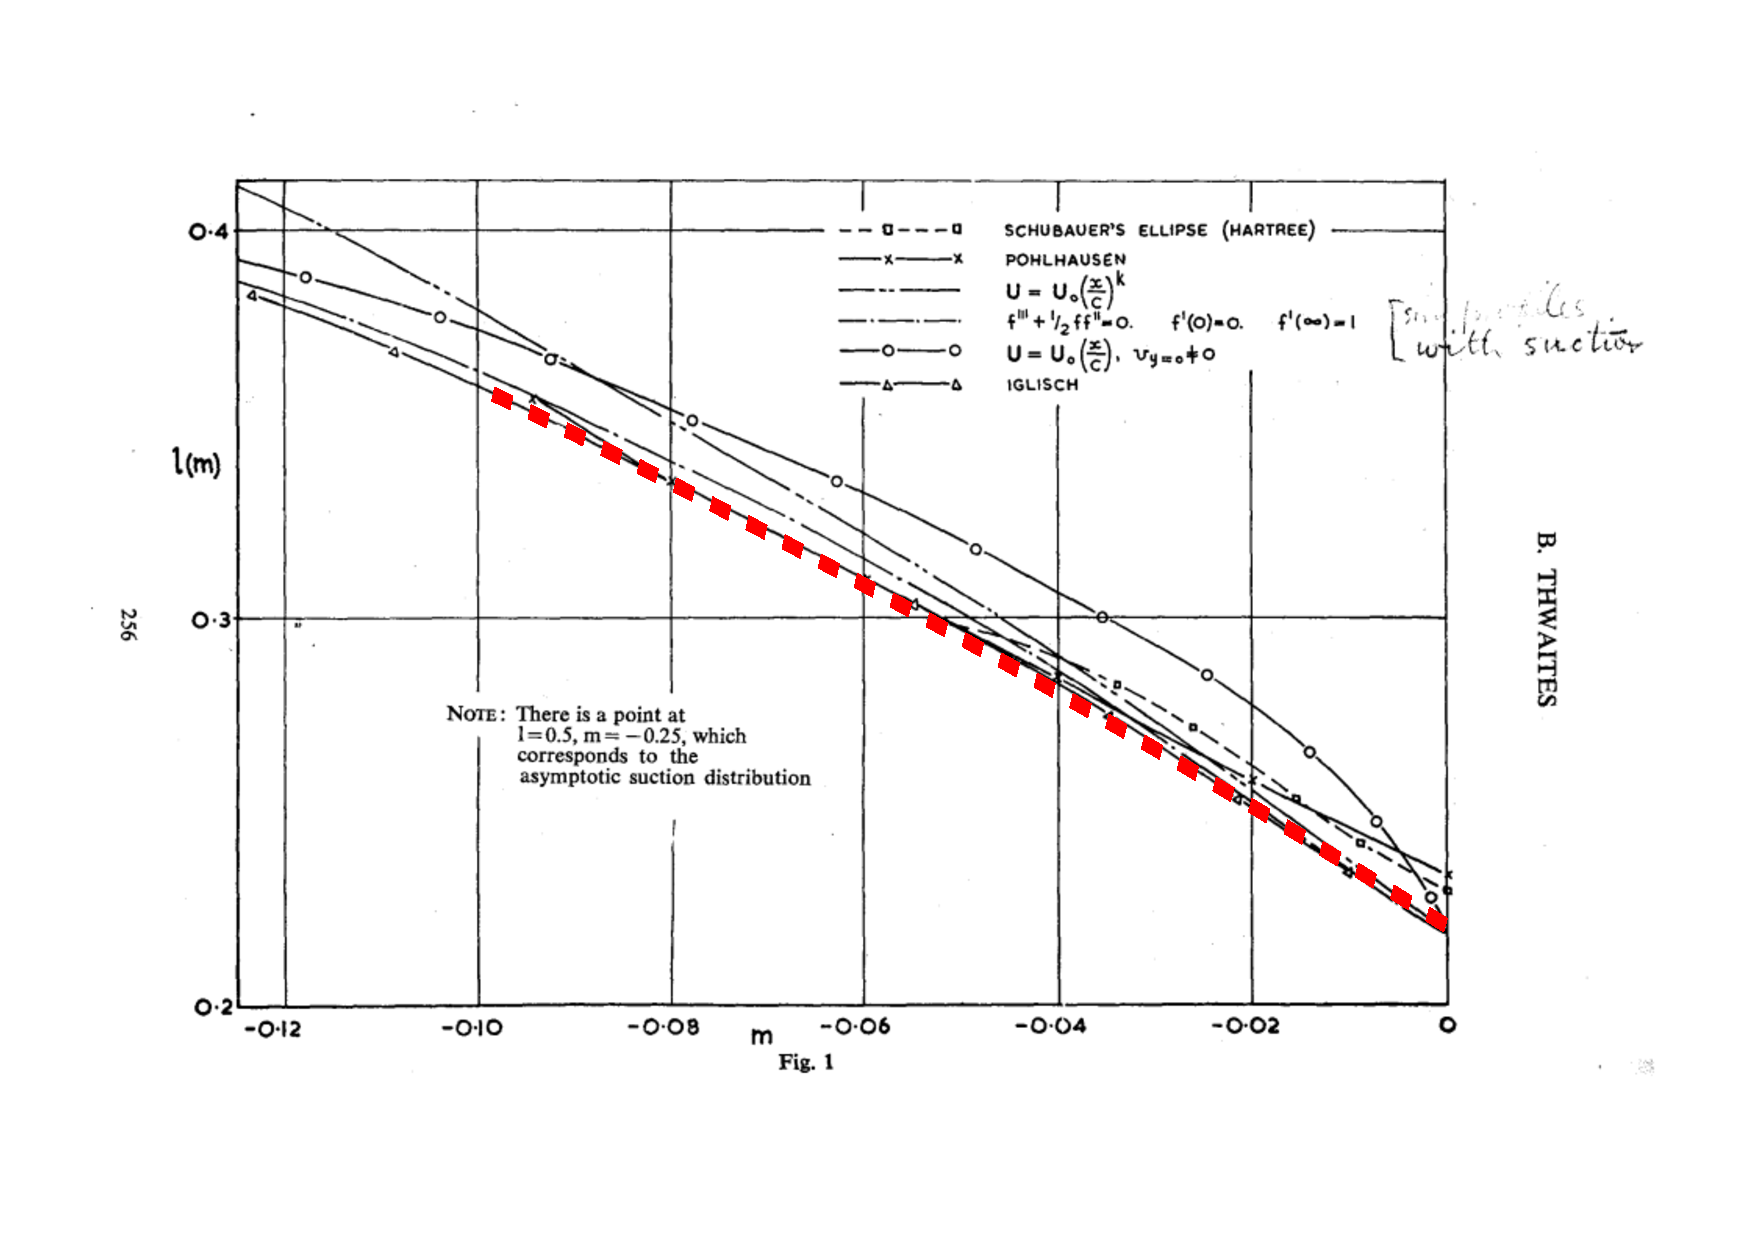
\includegraphics[width=0.95\textwidth, trim= 0  60 0  50, clip]{./../template/fig/cfr_ell_m_neg}
\caption{$\ell(m)$, per correnti accelerate, $m<0$.}\label{fig:ell_m_neg}
\end{figure}

\begin{figure}[h!]
\centering
 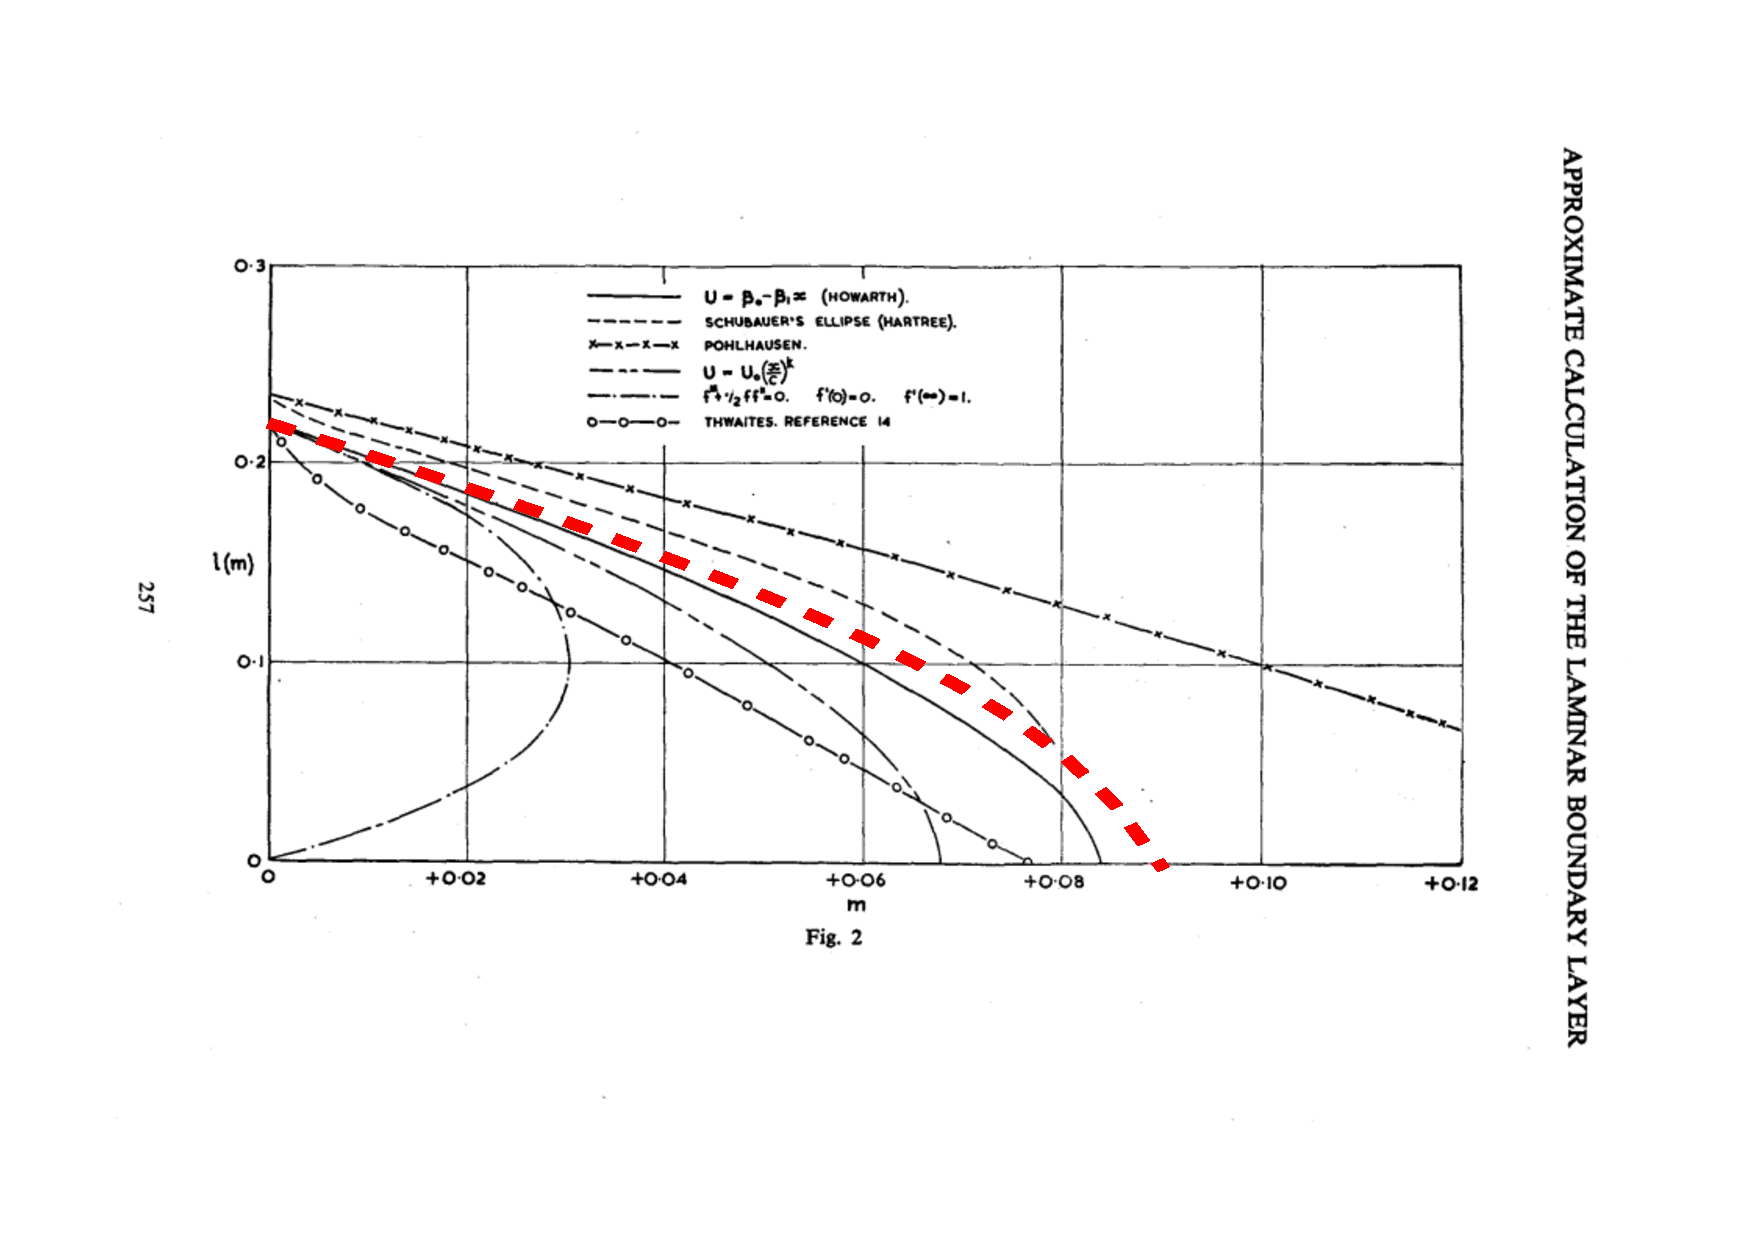
\includegraphics[width=0.95\textwidth, trim= 0  60 0 100, clip]{./../template/fig/cfr_ell_m_pos}
\caption{$\ell(m)$, per correnti con gradiente di pressione avverso, $m>0$.}\label{fig:ell_m_pos}
\end{figure}

\begin{figure}[h!]
\centering
 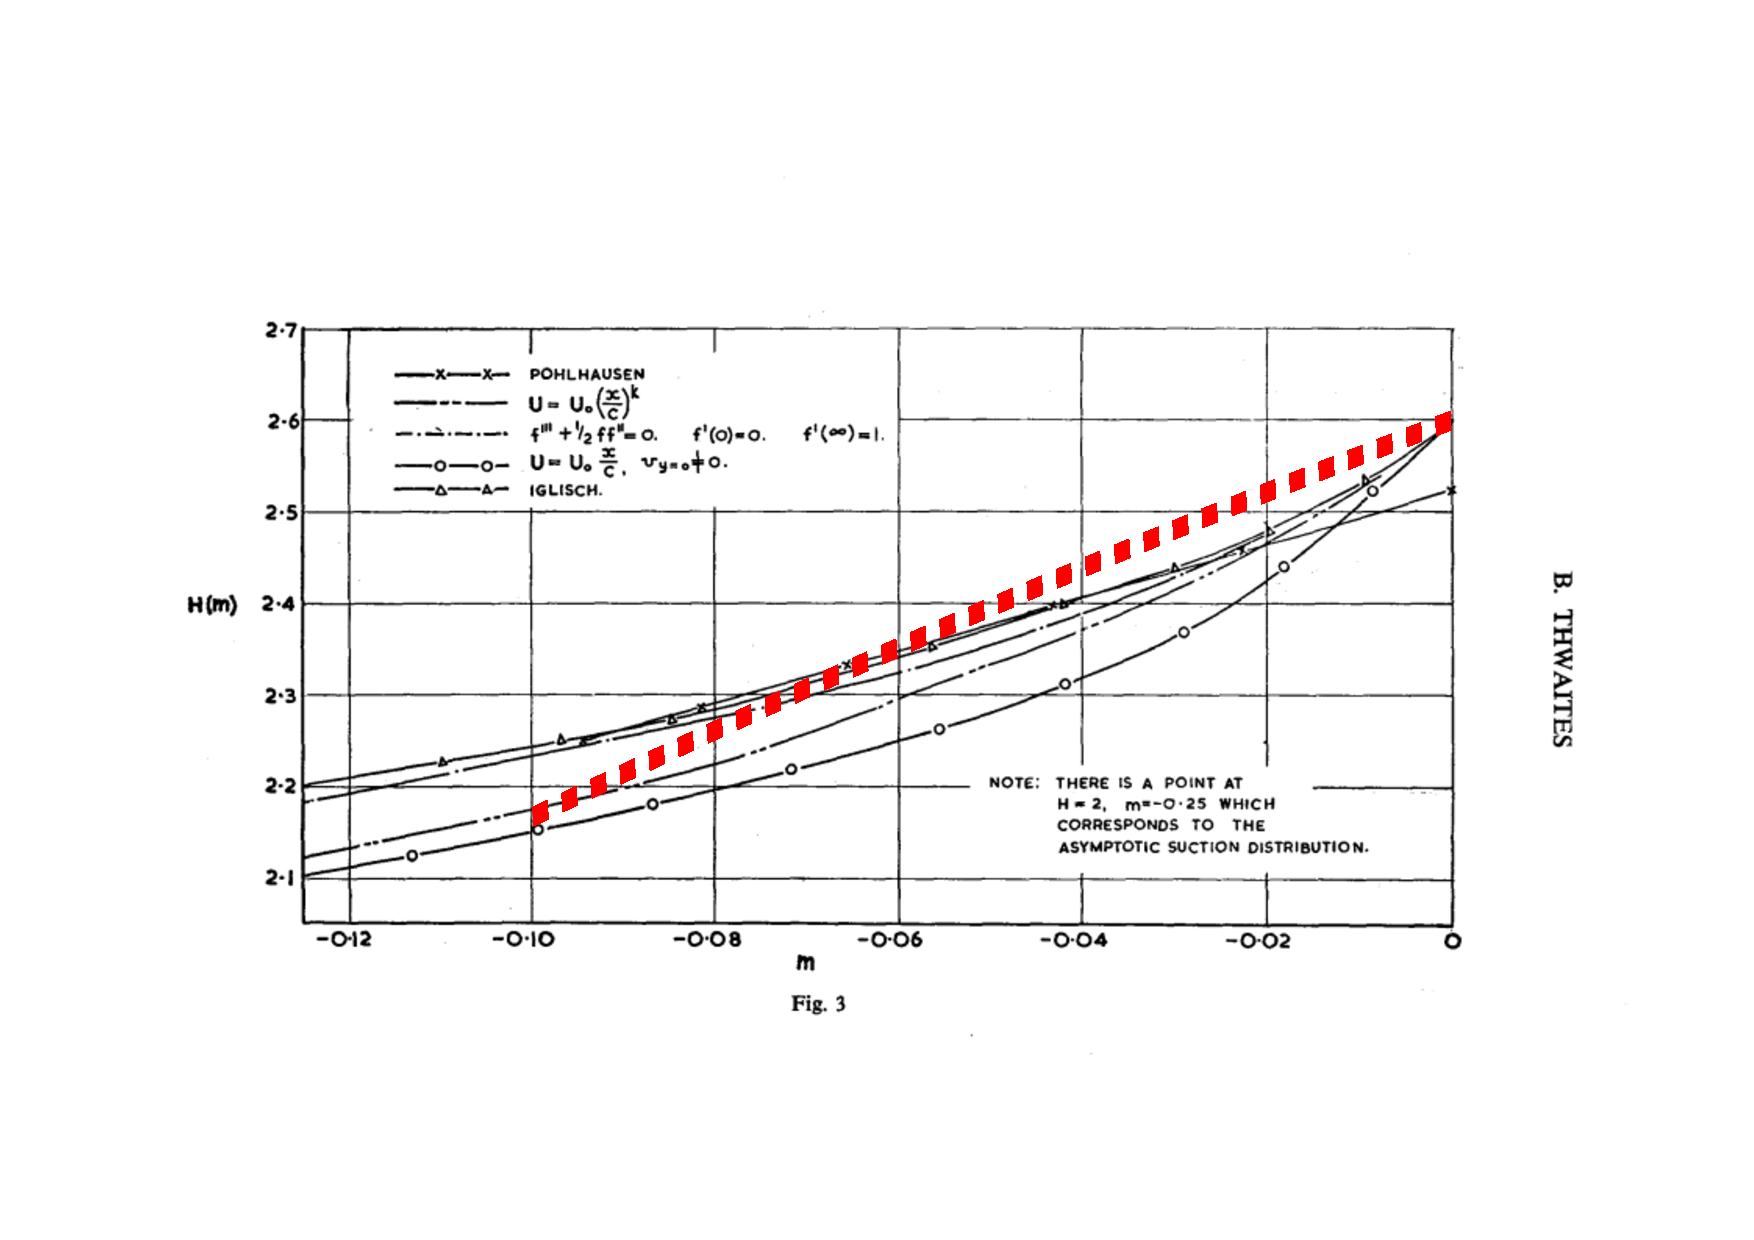
\includegraphics[width=0.95\textwidth, trim= 0 120 0 100, clip]{./../template/fig/cfr_H_m_neg}
\caption{$H(m)$, per correnti accelerate, $m<0$.}\label{fig:H_m_neg}
\end{figure}

\begin{figure}[h!]
\centering
 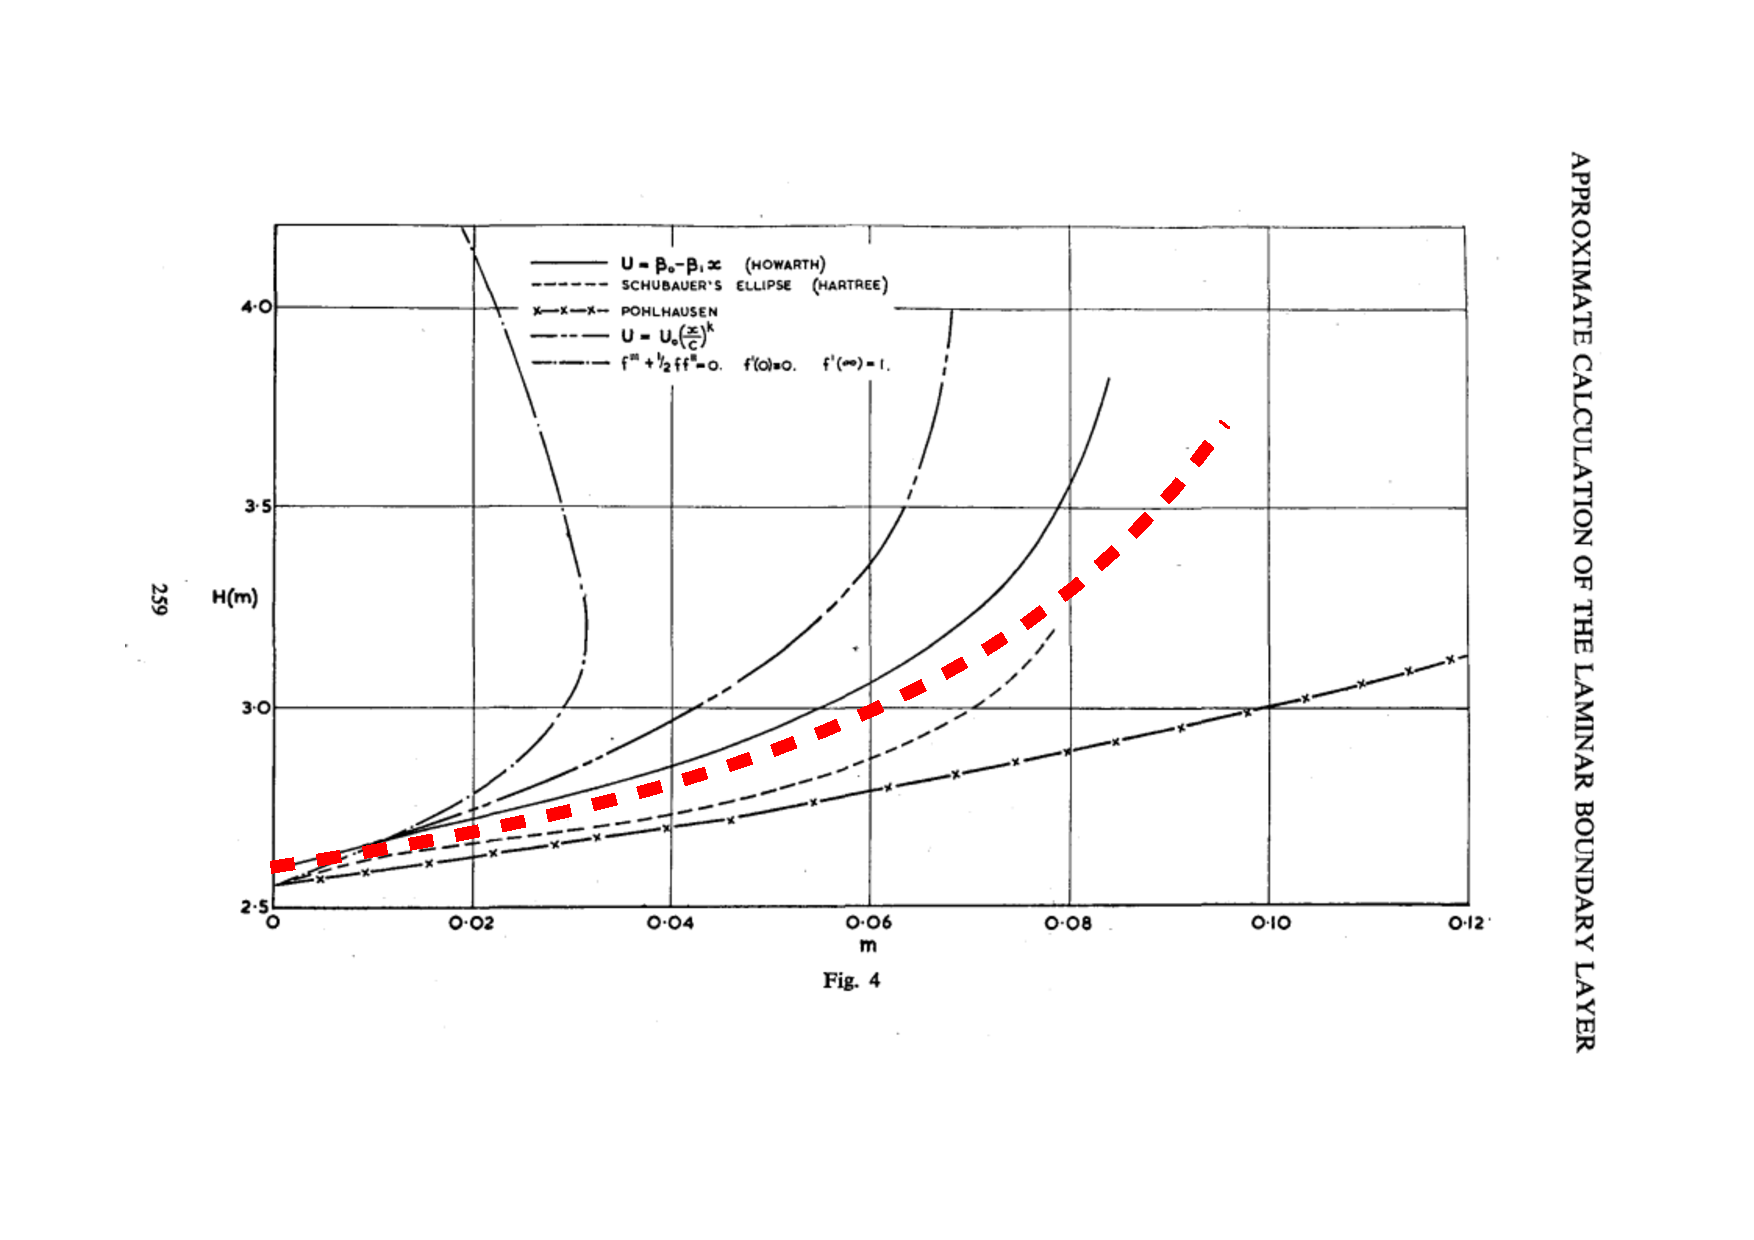
\includegraphics[width=0.95\textwidth, trim= 0  90 0 100, clip]{./../template/fig/cfr_H_m_pos}
\caption{$H(m)$, per correnti con gradiente di pressione avverso, $m>0$.}\label{fig:H_m_pos}
\end{figure}


\paragraph{Metodo di Thwaites ed equazione integrale di Von Karman.}
Si può manipolare l'equazione integrale di Von Karman (\ref{eqn:vkie}) per far comparire lo sforzo a parete $\tau_w$ e il gradiente di pressione $dP/dx$ prima, e i numeri adimensionali utilizzati da Thwaites $\ell$, $m$ poi.
%
Utilizzando la definizione del coefficiente di attrito,
\begin{equation}
 c_f := \dfrac{\tau_w}{\frac{1}{2}\rho U^2} \ ,
\end{equation}
e utilizzando il teorema di Bernoulli per legare la variazione della velocità esterna alla variazione della pressione,
\begin{equation}
 \rho U(x) \dfrac{dU}{dx}(x) = - \dfrac{dP}{dx}(x) \ ,
\end{equation}
si può riscrivere l'equazione di Von Karman come
\begin{equation}
\begin{aligned}
 \dfrac{d\theta}{dx} & = \dfrac{\tau_w}{\rho U^2} + ( 2 + H ) \dfrac{\theta}{\rho U^2}\dfrac{dP}{dx} = \\
  & = \dfrac{1}{\rho U^2} \left[ \dfrac{\mu U}{\theta} \, \ell + ( 2 + H ) \dfrac{\theta}{\rho U^2} \dfrac{\mu U}{\theta^2} \, m \right] = \\
  & = \dfrac{\nu}{U\theta} \left[  \ell + ( 2 + H ) \, m \right] \ .
\end{aligned}
\end{equation}
Secondo le ipotesi fatte da Thwaites, $\ell(m)$ e $H(m)$, il contenuto della parentesi quadra può essere scritto come una funzione di $m = \dfrac{dP}{dx} \dfrac{\theta^2(x)}{\mu U(x)}$,
\begin{equation}\label{eqn:vkie:2}
 \dfrac{U\theta}{\nu} \dfrac{d\theta}{dx} = [ \ell(m) + ( 2 + H(m) ) \, m ] =: \dfrac{L(m)}{2} \ .
\end{equation}
Conoscendo la distribuzione di velocità $U(x)$ e pressione $P(x)$ esterna, e l'espressione delle funzioni $\ell(m)$, $H(m)$, questa equazione contiene solo la funzione $\theta(x)$ come incognita, ed è integrabile (numericamente), una volta nota una condizione iniziale $\theta(x_0) = \theta_0$.

\paragraph{Linearizzazione di $L(m)$.} Nell'intorno di $m=0$, condizione di gradiente di pressione nullo, si può ottenere un'approssimazione affine della funzione $L(m)$,
\begin{equation}
 L(m) \approx 0.45 + 6 \, m \ .
\end{equation}
Inserendo questa approssimazione nell'equazione (\ref{eqn:vkie:2}), si ottiene
\begin{equation}\label{eqn:vkie:3}
 2 \dfrac{U(x) \theta(x)}{\nu} \dfrac{d \theta}{dx} = 0.45 - 6 \dfrac{\theta^2(x)}{\nu} \dfrac{dU}{dx} \ ,
\end{equation}
avendo espresso il parametero $m$ in funzione della variazione della velocità esterna,
\begin{equation}
 m = \dfrac{dP}{dx} \dfrac{\theta^2}{\mu U} = - \dfrac{\theta^2}{\nu} \dfrac{dU}{dx} \ .
\end{equation}
Moltiplicando l'equazione (\ref{eqn:vkie:3}) per $U^5(x)$, si può riscrivere
\begin{equation}
 \dfrac{d}{dx} \left( \theta^2 U^6 \right) = \nu U^5 \ ,
\end{equation}
pronta per essere integrata come
\begin{equation}
 U^6(x) \theta^2(x) - U^6(x_0) \theta^2(x_0) = 0.45 \, \nu \int_{\xi=0}^{x} U^5(\xi) d \xi \ ,
\end{equation}
da dove ricavare lo spessore integrale della quantità di moto $\theta(x)$.

\paragraph{Ricostruzione delle altre grandezze fisiche.}
Una volta calcolato $\theta(x)$, si può calcolare il parametro $m(x)$ lungo il corpo
\begin{equation}
  m = - \dfrac{\theta^2(x)}{\nu}\dfrac{dU}{dx}(x) \ ,
\end{equation}
con il quale calcolare gli altri parametri adimensionali,
\begin{equation}
 \ell(x) = \ell(m(x)) \qquad , \qquad H(x) = H(m(x)) \ ,
\end{equation}
con i quali calcolare lo sforzo a parete e lo spessore di spostamento
\begin{equation}
 \tau_w(x) = \ell(x) \dfrac{\mu U(x)}{\theta(x)} \qquad , \qquad \delta^*(x) = H(x) \theta(x) \ .
\end{equation}

\subsection{Criteri di transizione}
{\color{red} TODO: criterio di transizione di Michel.}
Per una corretta stima della resistenza di attrito, è fondamentale essere in grado di descrivere la transizione dal regime laminare al regime turbolento, che hanno caratteristiche profondamente diverse.

\subsection{Metodo di Head per lo strato limite turbolento}
{\color{red} TODO: metodo di Head per lo strato limite turbolento}


% \vspace{10cm}
% 
% Utilizzando la definizione del coefficiente di attrito,
% \begin{equation}
%  c_f := \dfrac{\tau_w}{\frac{1}{2}\rho U^2} = 2 \dfrac{\nu}{U^2} \p{u}{y}\bigg|_{y=0} \ ,
% \end{equation}
% e la componente parallela alla parete della quantità di moto, valutata a parete,
% \begin{equation}
% 0 = \left[ u\p{u}{x} + v\p{u}{y} - \nu \dfrac{\partial^2 u}{\partial y^2} - U \f{dU}{dx}\right]\bigg|_{y=0} \qquad \rightarrow \qquad \nu \dfrac{\partial^2 u}{\partial y^2}\bigg|_{y=0} = - U \f{dU}{dx}  \ ,
% \end{equation}
% si può riscrivere l'equazione di Von Karman,
% \begin{equation}
%  \f{d\theta}{dx} - (2+H) \f{\theta}{U^2} \nu \dfrac{\partial^2 u}{\partial y^2}\bigg|_{y=0} =
%  \dfrac{\nu}{U^2} \p{u}{y}\bigg|_{y=0} \ ,
% \end{equation}
% e moltiplicando per il fattore $U \theta / \nu$,
% \begin{equation}
%  \f{U \theta}{\nu} \f{d\theta}{dx} =
%  \f{\theta}{U}\p{u}{y}\bigg|_{y=0} + (2+H) \f{\theta^2}{U} \dfrac{\partial^2 u}{\partial y^2}\bigg|_{y=0} \ .
% \end{equation}
% Seguendo Thwaites, vengono definiti due parametri adimensionali,
% \begin{equation}
%  \ell := \f{\theta}{U}\p{u}{y}\bigg|_{y=0} 
%  \qquad , \qquad
%     m := \f{\theta^2}{U} \dfrac{\partial^2 u}{\partial y^2}\bigg|_{y=0}
%        = - \dfrac{\theta^2}{\nu}\dfrac{dU}{dx} \ ,
% \end{equation}
% e l'equazione integrale di Von Karman diventa
% \begin{equation}
%  \f{U}{\nu} \f{d}{dx}\f{\theta^2}{2} = \ell + ( 2 + H ) m =: L(m) \ ,
% \end{equation}
% avendo introdotto la funzione $L(m)$, per la quale si può trovare una correlazione di dati sperimentali,
% \begin{equation}
%  L(m) = 0.45 + 6 \, m  \ .
% \end{equation}
% Utilizzando questa espressione della funzione $L(m)$ e la definizione di $m$ in termini della derivata della velocità esterna, l'equazione di Von Karman diventa
% \begin{equation}
%  \f{U}{\nu} \f{d}{dx}\f{\theta^2}{2} = 0.45 - 6 \f{\theta^2}{\nu}\f{dU}{dx} \ ,
% \end{equation}
% Portando a sinistra dell'uguale l'ultimo termine, moltiplicando tutti i termini dell'equazione per $U^5$, e sfruttando la regola di derivazione del prodotto, si può scrivere
% \begin{equation}
%  \f{d}{dx} \left( U^6 \theta^2 \right) = 0.45 \nu U^5 \ ,
% \end{equation}
% il cui integrale vale
% \begin{equation}
%  U^6(x)\theta^2(x) - U^6(x_0)\theta^2(x_0) = 0.45 \nu \int_{\xi=0}^{x} U^5(\xi) d\xi \ .
% \end{equation}
% Se si integra questa equazione a partire da un punto $x_0$ dove la velocità esterna è nulla, $U(x_0)^2$, si può trovare l'andamento dello spessore integrale della quantità di moto,
% \begin{equation}
%  \theta^2(x) = 0.45 \nu \f{1}{U^5(x)} \int_{\xi=0}^{x} U^5(\xi) d\xi \ .
% \end{equation}
% 
